\documentclass[addpoints]{physlabs}

\labtitle{Ohm's Law and Superconductivity}
\labnum{9}
\labnumroman{IX}
\course{PHYSICS 114 - 122 - 142 - 182}
\coursesubtitle{Electricity and Magnetism}
\date{\today}

\usetikzlibrary{patterns, angles, quotes, shapes, shapes.geometric, arrows.meta, decorations.pathmorphing, hobby}

% Gray table column type
\newcolumntype{g}{>{\columncolor{gray!20}}c}

\begin{document}

\maketitle

% PRELAB SECTION
\begin{prelab}

    \filbreak
    \question[1] Define the \textsl{critical temperature} for a superconducting material. Explain in words any method for measuring the critical temperature in a superconductor.
    %
    \begin{solution}[6cm]
        
    \end{solution}

    \filbreak
    \question[1] What is an ammeter? a voltmeter? What is the major difference in the way one uses each to measure electrical quantities in a simple electronic circuit? Be specific.
    %
    \begin{solution}[6cm]
        
    \end{solution}
        
\end{prelab}

% LAB SECTION
\begin{labsection}

\begin{objective}
    In the first part of this experiment, you will observe a fundamental property of superconductors, the levitation of a magnet by a superconductor, illustrating the Meissner Effect. In the second part of the experiment, you will observe and verify Ohm’s Law in simple resistive circuits.
\end{objective}

\begin{theory}

\subsection*{Ohm's Law and Equivalent Resistance}

In resistive circuits, Ohm's law governs the relationship between voltage, current, and resistance. Ohm's law states that if one applies a driving voltage $V$ to a circuit, the electrical current $I$ inside the circuit will be linearly proportional to $V$:
%
\begin{equation}\label{eq: Ohm's law}
    V = IR.
\end{equation}
%
The constant of proportionality $R$ in eq.~\ref{eq: Ohm's law} is the resistance of the circuit.

Simple electronic circuits can be made using a direct-current (DC) voltage supply, such as a battery or a bench supply, which provides a constant potential difference between two junctions in a circuit. The DC voltage supply is connected to a combination of low-resistance wires, individual resistive elements called \textbf{resistors}, and (perhaps) measurement devices such as voltmeters and ammeters to measure voltage and current, respectively.

Commonly-used resistors are carbon-based and come color-coded to enable easy visual identification of the resistance. As shown in Figure~\ref{fig: resistor combinations}, resistors can be combined in \textbf{parallel} combinations that divide the current into several branches, as well as \textbf{series} combinations in a single branch. (Other combinations are possible, of course, but we will not investigate them in this experiment.)

\begin{figure}[ht]
    \centering
    \begin{circuitikz}
        % Parallel circuit
        \begin{scope}[shift={(6,0)}]
            \draw (0,0) coordinate (O)
                  to[short, o-*] ++(1,0) coordinate (A)
                  to[R, l^=$R_2$, -*] ++(3,0) coordinate (B)
                  to[short, -o] ++(1,0);
            \draw (A) to[short] ++(0,1.25)
                  to[R, l^=$R_1$] ++(3,0)
                  to[short] (B);
            \draw (A) to[short] ++(0,-1.25)
                  to[R, l^=$R_3$] ++(3,0)
                  to[short] (B);
            \draw (2.5,-2) node {parallel combination};
        \end{scope}
        % Series circuit
        \begin{scope}[shift={(0,-1.25)}]
            \draw (0,0) coordinate (O)
                  to[R, l^=$R_1$, o-] ++(0,2.5)
                  to[R, l^=$R_2$] ++(3,0)
                  to[R, l^=$R_3$, -o] ++(0,-2.5);
            \draw (1.5,-0.75) node {series combination};
        \end{scope}
    \end{circuitikz}
    \caption{A set of three resistors combined in series (left) and in parallel (right).}
    \label{fig: resistor combinations}
\end{figure}

Resistors combined in this manner can be expressed as a single combined or equivalent resistance $R_\text{eq}$. Resistors combined in series have an equivalent resistance that is just the sum of the individual resistances. For resistors combined in parallel, the inverse of the equivalent resistance is equal to the sum of the individual inverse resistances.

\begin{align}
    &\text{Series} & R_\text{eq} &= R_1 + R_2 + R_3 + \ldots \label{eq: series resistance}
    \\
    &\text{Parallel} & \frac{1}{R_\text{eq}} &= \frac{1}{R_1} + \frac{1}{R_2} + \frac{1}{R_3} + \ldots \label{eq: parallel resistance}
\end{align}

\subsection*{Resistors in Series: A Voltage Divider}

A common application of resistors in series is in a device called a \textbf{voltage divider}. The divider does exactly what its name suggests: it takes a voltage input and successively steps down (or divides) the voltage by putting the input voltage across a set of resistors in series. This can be used to do useful things like adjust the level of a signal in a circuit, provide fixed bias voltages to output devices, etc.

\begin{wrapfigure}[14]{r}{0.35\linewidth}
    \centering
    \begin{circuitikz}
    \draw (0,0) coordinate (A)
          to[battery2, invert, l^=$V_s$] ++(0,5)
          to[short] ++(2.5,0) coordinate (B)
          to[R, l^=$R_1$] ++(0,-2.5) coordinate (C)
          to[R, l^=$R_2$] ++(0,-2.5) coordinate (D)
          to[rmeter, t=A] (A);
    % Draw currents
    \draw[red, -latex]
          ($ (A) + (0.75,2)$) -- node[midway, right] {$I_s$} ++(0,1);
    \draw[red, -latex]
          ($ (B) - (0.5,0.75)$) -- node[midway, left] {$I_1$} ++(0,-1);
    \draw[red, -latex]
          ($ (C) - (0.5,0.75)$) -- node[midway, left] {$I_2$} ++(0,-1);
    % Draw leads to voltmeters measuring V1 and V2
    \draw[gray] ($ (B) - (0,0.25)$)
          to[short, *-] ++(1.5,0)
          to[short] node[pos=0.5,fill=white] {$V_1$} ++(0,-2)
          to[short, -*] ++(-1.5,0);
    \draw[gray] ($ (C) - (0,0.25)$)
          to[short, *-] ++(1.5,0)
          to[short] node[pos=0.5,fill=white] {$V_2$} ++(0,-2)
          to[short, -*] ++(-1.5,0);
\end{circuitikz}
    \caption{A voltage divider.}
    \label{fig: voltage divider}
\end{wrapfigure}

An example voltage divider is shown in Figure~\ref{fig: voltage divider}. A power supply with voltage $V_s$ is connected across two resistors in series, $R_1$ and $R_2$. Let's do a simple analysis of the circuit.

\begin{enumerate}
    \item Notice that the current through $R_1$ and $R_2$ must be the same, because there is only one path through the circuit. Since the only current is $I_s$ from the power supply, we must have
    \[
        I_s = I_1 = I_2.
    \]

    \item The voltages around the loop must sum to zero (Kirchhoff's loop rule), so we must have
    \[
        V_s = V_1 + V_2.
    \]

    \item We can treat the two series resistance as the single equivalent resistance $R_\text{eq}=R_1+R_2$. Thus, by Ohm's law,
    \[
        V_s = I_s R_\text{eq} = I_s(R_1 + R_2).
    \]
\end{enumerate}
%
Putting these elements together, we find that the fraction of the voltage going through each resistor, in terms of the supply voltage $V_s$, is
%
\begin{align}\label{eq: voltage divider}
    V_1 &= V_s\frac{R_1}{R_1+R_2},
    &
    V_2 &= V_s\frac{R_2}{R_1+R_2}.
\end{align}
%
I.e., the voltage drop across each resistor is proportional to its resistance, divided by the equivalent series resistance. Thus, the series resistors divide the supply voltage along the chain of resistors.

\subsection*{Resistors in Parallel: A Current Divider}

\begin{wrapfigure}[14]{r}{0.35\linewidth}
    \centering
    \begin{circuitikz}
    \draw (0,0) coordinate (A)
          to[battery2, invert, l^=$V_s$] ++(0,3)
          to[rmeter, t=A] ++(0,2) coordinate (B)
          to[short, -*] ++(2,0) coordinate (C)
          to[R, l^=$R_1$] ++(0,-3) coordinate (D)
          to[rmeter, t=A, -*] ++(0,-2) coordinate (E)
          to[short] (A);
    \draw (C) to[short] ++(2,0)
          to[R, l^=$R_2$] ++(0,-3)
          to[rmeter, t=A] ++(0,-2)
          to[short] (E);
    % Draw currents
    \draw[red, -latex]
          ($ (A) + (0.5,2)$) -- node[midway, right] {$I_s$} ++(0,1);
    \draw[red, -latex]
          ($ (C) - (0.5,1)$) -- node[midway, left] {$I_1$} ++(0,-1);
    \draw[red, -latex]
          ($ (C) + (1.5,-1)$) -- node[midway, left] {$I_2$} ++(0,-1);
\end{circuitikz}
    \caption{A current divider.}
    \label{fig: current divider}
\end{wrapfigure}

In Figure~\ref{fig: current divider}, a voltage supply $V_s$ is connected across two resistors in parallel. We notice the following details:

\begin{enumerate}
    \item The current splits between the two branches of the circuit. By Kirchhoff's sum rule, the currents must sum to the current from the supply:
    \[
        I_s = I_1 + I_2.
    \]

    \item The voltage across the two resistors must be the same, because their endpoints are connected by a conducting wire with negligible resistance. Thus,
    \[
        V_s = V_1 = V_2.
    \]

    \item Using eq.~\ref{eq: parallel resistance} and Ohm's law, we find that
    \[
        V_s = I_s R_\text{eq} = I_s\frac{R_1R_2}{R_1+R_2}.
    \]
\end{enumerate}
%
Combining these results, it is straightforward to show that 
%
\begin{align}\label{eq: current divider}
    I_1 &= I_s\frac{R_2}{R_1+R_2},
    &
    I_2 &= I_s\frac{R_1}{R_1+R_2}.
\end{align}
%
I.e., the current in resistor 1 is proportional to $R_2$, and the current in resistor 2 is proportional to $R_1$. This hopefully makes intuitive sense. For example, if $R_1>R_2$, then $I_2>I_1$ because the resistance is lower in the second branch of the circuit, causing more current to flow through $R_2$.

\subsection*{Superconductivity}

At the microscopic scale, an electrically conducting material can be thought of as an atomic lattice with energy levels that allow electrons to move freely when a voltage is applied across the material. The electrons' collective motion gives rise to the macroscopic current we measure in the lab. As electrons move through the material, they scatter off the atomic lattice, converting their kinetic energy to vibrational energy in the lattice and heating the material. (This is why live wires are hot to the touch!) This ``frictional'' dissipation of energy is characterized by the resistivity of the material and is the origin of Ohm's law.

However, some materials called \textbf{superconductors} lose all measurable electrical resistivity at low temperatures. In a superconductor, even without any driving voltage, an electrical current will flow indefinitely with no discernible decay. This phenomenon was originally observed in 1911, when the Dutch physicist Heike Kamerlingh Onnes used liquid helium to cool solid mercury to \qty{1.5}{\kelvin}\footnote{Kamerlingh Onnes was the first person to liquefy helium, and he was awarded a Nobel Prize for this work in 1913.}. Kamerlingh Onnes observed that the electrical resistance of mercury rapidly drops to zero around \qty{4.2}{\kelvin}.

\subsubsection*{Critical Temperature}

Between 1911 and the mid-1980s, superconductivity was observed in a total of ten metals and alloys. 
In all cases, it was found that the transition from the normal resistive state to a superconducting non-resistive state occurs over a relatively small change in temperature. 
The temperature at which the transition occurs is called the \textbf{critical temperature} $T_C$, and its value depends on the material in question. 
Until the mid-1980s, the highest known critical temperature was $T_C=\qty{23}{\kelvin}$, for the niobium-germanium alloy \ce{Nb_3Ge}. 
In 1986 and 1987, a class of ceramic superconductors was discovered with $T_C=\qty{90}{\kelvin}$ to \qty{100}{\kelvin}. The discovery of such ``high-$T_C$'' superconductors\footnote{Georg Bednorz and K. Alex M\"{u}ller were awarded the Nobel Prize in 1987 for the discovery of high-$T_C$ ceramic superconductors.} is significant because $T_C$ is greater than the boiling temperature of liquid nitrogen (\qty{77}{\kelvin}), a common and inexpensive refrigerant.

Our theoretical understanding of superconductivity is incomplete. In 1957, John Bardeen, Leon Cooper, and J. Robert Schrieffer modeled superconducting current as the resistance-free transport of bound pairs of electrons (``Cooper pairs'') through the superconductor\footnote{Bardeen, Cooper, and Schrieffer were awarded the Nobel Prize for their theoretical work on superconductivity in 1972.}. This so-called BCS theory, named after the authors, cannot describe the high-$T_C$ superconductors, whose behavior is still not well-understood.

\subsubsection*{The Meissner Effect}

\begin{wrapfigure}{r}{0.35\linewidth}
    \centering
    
\includegraphics[width=0.9\linewidth]{Lab 09: Superconductivity and Ohm's Law/meissner-effect.png}
    \caption{At high $T$, a $B$ field penetrates a conductor (left), but the field is expelled below the superconducting transition (right). Credit: P. Jaworski, Wikimedia Commons.}
    \label{fig: Meissner effect}
\end{wrapfigure}

In addition to being \textbf{perfect conductors}, superconductors are \textbf{perfectly diamagnetic}. That is, when $T<T_C$, they expel magnetic fields from the interior of the material. An external magnetic field that tries to penetrate the superconductor is perfectly canceled by an opposing field produced by superconducting currents inside the material. A diagram of this effect is shown in Figure~\ref{fig: Meissner effect}. The expulsion of magnetic fields from superconductors, first observed by Walther Meissner and Robert Ochsenfeld in 1933, is called the Meissner effect.

If the external field comes from a magnet, the expulsion of the field lines produces a repulsive force on the magnet. Thus, a magnet positioned above the superconductor will be levitated, a phenomenon that you will investigate in this experiment.

Practical, real-world examples of the Meissner effect are its use in magnetic suspension systems, where it is desirable to eliminate mechanical friction (in maglev trains, for example) or to provide mechanical stability in applications using strong magnetic fields (e.g., magnetic resonance imaging).

\end{theory}

\begin{experiment}

\subsection*{Ohm's Law}

\begin{center}
\setlength{\fboxsep}{6pt}%
\setlength{\fboxrule}{2pt}%
\fbox{\begin{minipage}{0.9\textwidth}
    \color{RoyalBlue}
    Note: students at \textbf{EVEN}-numbered tables will do Ohm's law first, and superconductivity second. Students at \textbf{ODD}-numbered tables should skip to superconductivity and do this section second. 
\end{minipage}}
\end{center}

\subsubsection*{A Note about Resistor Color Codes}

Carbon composition resistors (CCRs) of the type you will use are made with hundreds of different resistance values, tolerances, and power ratings. They are very inexpensive and bought in bulk, and in an electronics stockroom, it is common to find drawers filled with hundreds to thousands of different resistors. To keep things straight, the value of a resistor may be read from a code of color bands printed on its exterior, as shown in Figure~\ref{fig: resistor color code}. In the lab, you will typically see resistors with four bands, although 3-band, 5-band, and 6-band codes are also used.

\begin{figure}[ht]
    \centering
    % \Stripe{offset}{color} long stripe
\newcommand\Stripe[2]{\draw[fill=#2,#2] ++(#1,0) +(-0.15,-0.71) rectangle +(0.15,0.71);}
% \stripe{offset}{color} short stripe
\newcommand\stripe[2]{\draw[fill=#2,#2] ++(#1,0) +(-0.15,-0.51) rectangle +(0.15,0.51);}

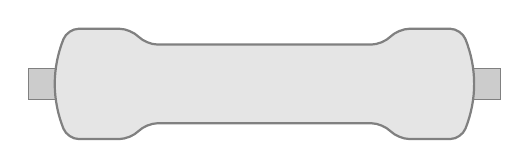
\begin{tikzpicture}
    % wire
    \draw[gray,fill=gray!40] (-3,-0.2) rectangle (3,0.2);
    % resistor
    \draw[rounded corners,thick,gray,fill=gray!20]
    ++(0,0.5) -- ++(1.5,0) -- ++(0.2,0.2) -- ++(0.8,0)
    .. controls +(0.2,-0.5) and +(0.2,0.5) .. ++(0,-1.4) -- ++(-0.8,0)
    -- ++(-0.2,0.2) -- ++(-3,0) -- ++(-0.2,-0.2) -- ++(-0.8,0)
    .. controls +(-0.2,0.5) and +(-0.2,-0.5) .. ++(0,1.4) -- ++(0.8,0)
    -- ++(0.2,-0.2) -- cycle;
    \Stripe{-2.1}{red!80!gray}
    \Stripe{2.1}{yellow!50!gray}
    \stripe{-1.2}{RoyalBlue}
    \stripe{-0.4}{brown}
\end{tikzpicture}
    \caption{Color codes for a \qty{260}{\ohm} resistor with 5\% tolerance.}
    \label{fig: resistor color code}
\end{figure}

Figure~\ref{fig: resistor color code} is a 4-band resistor. To read the code, start from the first color band where the bands are bunched at one end (in this case, the red band). The first two bands represent the first two digits in the value of $R$. The third color band represents a multiplier to yield the final resistance value in ohms. If there is a fourth band present, it is a measure of the tolerance of the resistor, giving the uncertainty in the resistor's printed resistance value.

\begin{table}[ht]
    \centering
    \caption{Resistor color codes (4-band resistors)}
    \label{tab: resistor color code}
    \renewcommand{\arraystretch}{1.2}
    \rowcolors{2}{white}{gray!10}
    \begin{tabular}{|l|>{\centering\arraybackslash}p{1.5cm}|>{\centering\arraybackslash}p{1.5cm}|c|c|}
        \hline
        \multicolumn{1}{|c|}{\textbf{Color}} & \multicolumn{2}{|c|}{\textbf{Significant Figures}} & \textbf{Multiplier} & \textbf{Tolerance}
        \\
        \hline
        
\begin{tikzpicture}\filldraw[black] (0,0) rectangle (0.5,0.2); \end{tikzpicture}\ \ black & 0 & 0 & $\times1$ &
        \\
        \hline
        
\begin{tikzpicture}\filldraw[brown] (0,0) rectangle (0.5,0.2); \end{tikzpicture}\ \ brown & 1 & 1 & $\times10$ & $\pm1\%$ (F)
        \\
        \hline
        
\begin{tikzpicture}\filldraw[red] (0,0) rectangle (0.5,0.2); \end{tikzpicture}\ \ red & 2 & 2 & $\times100$ & $\pm2\%$ (G)
        \\
        \hline
        
\begin{tikzpicture}\filldraw[orange] (0,0) rectangle (0.5,0.2); \end{tikzpicture}\ \ orange & 3 & 3 & $\times\qty{1}{\kilo\nothing}$ & $\pm0.05\%$ (G)
        \\
        \hline
        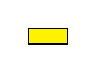
\begin{tikzpicture}\draw[fill=yellow] (0,0) rectangle (0.5,0.2); \end{tikzpicture}\ \ yellow & 4 & 4 & $\times\qty{10}{\kilo\nothing}$ & $\pm0.02\%$ (P)
        \\
        \hline
        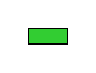
\begin{tikzpicture}\draw[fill=LimeGreen] (0,0) rectangle (0.5,0.2); \end{tikzpicture}\ \ green & 5 & 5 & $\times\qty{100}{\kilo\nothing}$ & $\pm0.5\%$ (D)
        \\
        \hline
        
\begin{tikzpicture}\filldraw[RoyalBlue] (0,0) rectangle (0.5,0.2); \end{tikzpicture}\ \ blue & 6 & 6 & $\times\qty{1}{\mega\nothing}$ & $\pm0.25\%$ (C)
        \\
        \hline
        
\begin{tikzpicture}\filldraw[violet] (0,0) rectangle (0.5,0.2); \end{tikzpicture}\ \ violet & 7 & 7 & $\times\qty{10}{\mega\nothing}$ & $\pm0.1\%$ (B)
        \\
        \hline
        
\begin{tikzpicture}\filldraw[gray] (0,0) rectangle (0.5,0.2); \end{tikzpicture}\ \ gray & 8 & 8 & $\times\qty{100}{\mega\nothing}$ & $\pm0.01\%$ (L)
        \\
        \hline
        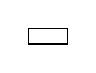
\begin{tikzpicture}\draw[fill=white] (0,0) rectangle (0.5,0.2); \end{tikzpicture}\ \ white & 9 & 9 & $\times\qty{1}{\giga\nothing}$ &
        \\
        \hline
        
\begin{tikzpicture}\filldraw[yellow!50!gray] (0,0) rectangle (0.5,0.2); \end{tikzpicture}\ \ gold &  &  & $0.1$ & $\pm5\%$ (J)
        \\
        \hline
        
\begin{tikzpicture}\filldraw[gray!50] (0,0) rectangle (0.5,0.2); \end{tikzpicture}\ \ silver &  &  & $0.01$ & $\pm10\%$ (K)
        \\
        \hline
    \end{tabular}
\end{table}

To read the resistance shown in Fig.~\ref{fig: resistor color code}, refer to Table~\ref{tab: resistor color code}. The first two bands (red and blue) represent the numbers 2 and 6. The third band (brown) represents the multiplier $10$. The fourth band (gold) represents a tolerance of 5\%. Thus, the resistance is
\[
    R = 26\times10 = \qty{260}{\ohm} \pm 5\% = \qty{260}{\ohm} \pm \qty{13}{\ohm}.
\]
Thus, if you connect a digital multimeter to the resistor and measure its resistance, you should expect to read a value in the range of about \qty{247}{\ohm} to \qty{273}{\ohm}.

\subsubsection*{A Single Resistor: Procedure}

\begin{wrapfigure}{r}{0.4\linewidth}
    \centering
    \begin{circuitikz}
        \draw (0,0) coordinate (A)
              to[battery2, invert, l^=$V_s$] ++(0,3) coordinate (B)
              to[short] ++(2,0) coordinate (C)
              to[R, l^=$R$] ++(0,-3) coordinate (D)
              to[rmeter, t=A] (A);
        % Draw leads to voltmeters measuring V
        \draw ($ (C) - (0,0.25)$)
              to[short, *-] ++(1.5,0)
              to[rmeter, t=V] ++(0,-2.5)
              to[short, -*] ++(-1.5,0);
    \end{circuitikz}
    \caption{A single-resistor circuit.}
    \label{fig: single resistor}
\end{wrapfigure}

Connect your electronic components into a single-resistor circuit as shown in Figure~\ref{fig: single resistor}. The voltmeter (circled ``V'') does not interrupt the flow of current in the circuit; it measures the potential difference across the resistor $R$. On the other hand, the ammeter (circled ``A'') measures current, so it needs to interrupt the flow of the circuit.

In other words, you must have one wire leave the output of the power supply and go to the resistor. A wire will leave the other end of the resistor and go into the milliamp
(mA) port of the ammeter. Another wire will exit the Common/Ground port of the ammeter and return to the ground of the power supply. The voltmeter will have 2 wires connected to it: one wire will tap into one side of the resistor, and the other wire will tap into the opposite end of the resistor. Use a resistor of at least \qty{1000}{\ohm}. Use the color code in Table~\ref{tab: resistor color code} to select the correct resistor.

\begin{enumerate}
    \item Raise the supply voltage $V_s$ from \qty{0}{\volt} to \qty{10}{\volt} in steps of \qty{1}{\volt}, taking readings of the voltage and current at each step and recording them in Data Table~\ref{data: single resistor}.

    Note: if you get negative values for voltage or current, disregard the minus sign and just record the number.

    \item Continue measuring until you have 10 data points ranging from \qty{1}{\volt} to \qty{10}{\volt}.

    \item Measure the resistance of $R$ using the ohmmeter capability of the digital multimeter. Record your data in Data Table~\ref{data: single resistor}.
\end{enumerate}

\subsubsection*{Does a Light Bulb Obey Ohm's Law? Procedure}

In this section, you will determine whether a common incandescent light bulb obeys Ohm's law. You will set up the light bulb in place of the resistor in the circuit shown in Fig.~\ref{fig: single resistor}.

\begin{center}
\setlength{\fboxsep}{6pt}%
\setlength{\fboxrule}{2pt}%
\fbox{\begin{minipage}{0.9\textwidth}
    \color{OrangeRed}
    CAUTION: after you substitute the light bulb for the resistor, you \textbf{MUST} change the ammeter wires to the highest current setting allowed. A failure to do so could blow the fuse in your multimeter, wasting your time while we find a replacement fuse. Ask your TA or TI if you are unsure of what to do. 
\end{minipage}}
\end{center}

\begin{enumerate}
    \item Raise the supply voltage $V_s$ from \qty{0}{\volt} to \qty{6}{\volt} in steps of \qty{0.6}{\volt}, taking readings of the voltage and current at each step and recording them in Data Table~\ref{data: light bulb}.
    
    \item You should have 10 pairs of data points ranging from \qty{0}{\volt} to \qty{6}{\volt}. In the Postlab exercises, explore whether or not there is a linear relationship between $V$ and $I$ for the bulb.
\end{enumerate}

\subsubsection*{A Voltage Divider with Series Resistors: Procedure}

Set up the circuit shown in Fig.~\ref{fig: voltage divider setup}, using a \qty{220}{\ohm} in series with a \qty{1}{\kilo\ohm} resistor. You will also need to connect the ammeter in series between the resistors and the power supply ground. If you are still using the ammeter's high-current port from your measurements of the $I$-$V$ curve of the light bulb, switch your leads to use the low-current port. You will measure voltages across each of the two resistors using a voltmeter.

\begin{minipage}{0.5\linewidth}
    \centering
    \begin{circuitikz}
        \draw (0,0) coordinate (A)
              to[battery2, invert, l^=$\qty{3}{\volt}$] ++(0,5)
              to[short] ++(2.5,0) coordinate (B)
              to[R, l^=\qty{220}{\ohm}] ++(0,-2.5) coordinate (C)
              to[R, l^=\qty{1}{\kilo\ohm}] ++(0,-2.5) coordinate (D)
              to[rmeter, t=A] (A);
        % Draw leads to voltmeters measuring V1 and V2
        \draw ($ (B) - (0,0.25)$)
              to[short, *-] ++(2.5,0)
              to[rmeter, t=V] ++(0,-2)
              to[short, -*] ++(-2.5,0);
        \draw ($ (C) - (0,0.25)$)
              to[short, *-] ++(2.5,0)
              to[rmeter, t=V] ++(0,-2)
              to[short, -*] ++(-2.5,0);
    \end{circuitikz}
    \captionof{figure}{The circuit used to study a voltage divider.
    \label{fig: voltage divider setup}}
\end{minipage}
\begin{minipage}{0.5\linewidth}
    \centering
    \begin{circuitikz}
        \begin{scope}[shift={(0,0)}]
        \draw (0,0) coordinate (A)
              to[battery2, invert, l^=\qty{3}{\volt}] ++(0,3.25)
              to[rmeter, t=A] ++(0,2) coordinate (B)
              to[short, -*] ++(2,0) coordinate (C)
              to[R, l^=\qty{220}{\ohm}] ++(0,-2) coordinate (D)
              to[rmeter, t=A, -*] ++(0,-3.25) coordinate (E)
              to[short] (A);
        \draw (C) to[short] ++(2,0)
              to[R, l^=\qty{1}{\kilo\ohm}] ++(0,-2)
              to[rmeter, t=A] ++(0,-3.25)
              to[short] (E);
        \end{scope}
    \end{circuitikz}
    \captionof{figure}{The circuit used to study a current divider.
    \label{fig: current divider setup}}
\end{minipage}

\begin{enumerate}
    \item Set up your circuit as shown in Fig.~\ref{fig: voltage divider setup}. Use the resistor color codes in Table~\ref{tab: resistor color code} to choose a \qty{220}{\ohm} resistor and a \qty{1}{\kilo\ohm} resistor.
    \item Set the DC supply voltage to \qty{3}{\volt}.
    \item Measure the current $I_s$ from the supply and record the information in Data Table~\ref{data: series resistor}.
    \item Measure the voltage drop across each resistor using the voltmeter and record the result in Data Table~\ref{data: series resistor}.
    \item Record the actual values of each resistor in Data Table~\ref{data: series resistor}.
\end{enumerate}

\subsubsection*{A Current Divider with Parallel Resistors: Procedure}

\begin{enumerate}
    \item Assemble the circuit shown in Fig.~\ref{fig: current divider setup}.
    
    Note that if you don't have two ammeters to simultaneously measure the current in each branch, you will need to swap an ammeter between the branches. (\textbf{Don't forget to turn off the supply voltage before disconnecting and reconnecting elements in the circuit}.)

    \item Set the DC supply voltage to \qty{3}{\volt}.
    
    \item Using your current meter(s), measure the current from the supply voltage $I_s$, the current through the first resistor $I_1$, and the current through the second resistor $I_2$. Record your results in Data Table~\ref{data: parallel resistor}.
\end{enumerate}

\subsection*{Superconductivity}

\begin{center}
\setlength{\fboxsep}{6pt}%
\setlength{\fboxrule}{2pt}%
\fbox{\begin{minipage}{0.9\textwidth}
    \color{RoyalBlue}
    Note: students at \textbf{ODD}-numbered tables will do superconductivity first and Ohm's law second. Students at \textbf{EVEN}-numbered tables should do Ohm's law first, and this section second. 
\end{minipage}}
\end{center}

\subsubsection*{Safety Precautions}

In this measurement, you will be handling liquid nitrogen, which boils at \qty{77}{\kelvin} (\qty{-196.15}{\celsius}). 
The liquid nitrogen can cause severe ``burns'' due to its low temperature, so precautions must be taken. 
Read the following instructions carefully and follow all safety procedures. If you are unsure how to follow the safety procedures while doing this lab, please ask the lab TAs and TIs for help. \textbf{Those who do not follow the precautions will be removed from the lab and will not receive credit for the experiment.}

\begin{enumerate}
    \item Where safety glasses at all times in the presence of liquid nitrogen.
    \item Do not allow any liquid nitrogen to touch your body.
    \item Do not touch any items that have been immersed in liquid nitrogen until they warm to room temperature.
    \item Keep liquid nitrogen away from water -- it will flash boil and splash onto you.
    \item Be very careful to avoid overfilling or spilling liquid nitrogen from its container.
    \item Never store liquid nitrogen in a container with a tight-fitting lid. Pressure build-up from evaporating nitrogen can cause the container to explode.
    \item The superconductors are made of metal oxides that may be toxic, so only handle them with the tweezers provided. Never touch the superconductors with your bare hands, and wash your hands with soap and water after completing the experiment.
\end{enumerate}

\subsubsection*{Experimental Setup and Measurement Procedure}

The apparatus for exploring the Meissner effect using a YCBO superconductor is shown in Figure~\ref{fig: superconductor setup}. It consists of a foam bath with 9 terminals for connecting power supplies and measurement devices. Refer to the figure when making all connections.

\begin{figure}[ht]
    \centering
    \setlength{\fboxsep}{0pt}
    
\includegraphics[height=8cm]{Lab 09: Superconductivity and Ohm's Law/superconductor-setup.png}
    \hspace{1cm}
    \fbox{
\includegraphics[height=8cm]{Lab 09: Superconductivity and Ohm's Law/superconductor-connections.png}}
    \caption{Top-down view of the apparatus for studying the Meissner effect, with connection terminals labeled (left); photograph of the wired apparatus (right).}
    \label{fig: superconductor setup}
\end{figure}

\begin{enumerate}
    \item Set up a multimeter to measure DC voltage in the range \qty{20}{\milli\volt} and attach leads to terminals 3 and 4.

    \item Set up a second multimeter to measure DC voltage in the \qty{2}{\milli\volt} range and attach the leads to terminals 5 and 6.

    \item Set up third multimeter to measure current in the \qty{10}{\ampere} range. Do not use the \qty{200}{\milli\ampere} setting, or you could blow the fuse of the multimeter.

    \item Wire the terminals of a \qty{6}{\volt} battery to leads 1 and 2. Alternatively, set the DC power supply to 6V and wire the power supply's terminals to leads 1 and 2.

    \item Use the potentiometer (the blue box with a metal twist throttle located below leads 1 and 2) to set the current to a maximum of \qty{0.3}{\ampere}. Adjust the variable resistance as needed and make note of your final value in Data Table~\ref{data: critical temp} in the Postlab exercises.

    \item \textbf{Cooling}: Make sure the cork is secured in the foam and the aluminum foil tray is under the drainage pipe. Pour liquid nitrogen over the superconductor to bring the temperature below the critical temperature.
    
    \item You will measure its temperature with the voltmeter connected to leads 3 and 4, which will measure the superconductor's thermal conductivity. As the superconductor cools, the conductivity should go from about \qty{0}{\milli\volt} at room temperature to about \qty{6}{\milli\volt} when it is in equilibrium with the liquid nitrogen. When the multimeter connected to leads 5 and 6 reads \qty{0.0}{\milli\volt}, the superconductor is sufficiently cooled.

    \item Now, using a pair of tweezers, pick up one of the cubic magnets provided and place it on top of the superconductor disk. Try gently spinning the magnet with the tweezers. Observe whether the magnet is touching the surface of the disk, remembering to keep your fingers and your face from getting too close to the liquid nitrogen bath. Leave the cubic magnet there and continue to the next step.

    \item When you are ready to start taking data, use a cell phone camera to start a VIDEO RECORDING containing the values of all 3 meters. 
    Then \textbf{USE THE TWEEZERS} to remove the cork so the liquid nitrogen drains from the foam bath into the aluminum tray. 
    Be mindful not to accidentally touch the tray, which will get cold.

    \item Watch the Fluke meter's voltage, which is the thermal conductivity.
    If the thermal conductivity does not decrease after about a minute, aim an incandescent light bulb at the apparatus to speed up the warming process. 
    You may also start using the hair dryer on a low setting to warm up the system.

    \item  As the superconductor warms, keep recording the 3 meters' values. 
    Also, watch for the levitating magnet to fall and make a record (for instance by waving your hand in front of the camera) so you can record the temperature where this occurs.

    \item Once the thermal conductivity drops below 4 mV, stop the video recording.
    Disconnect the battery and various meters from the circuit. 
    Use a hairdryer on the ``low'' setting to evaporate any remaining liquid nitrogen in the foil tray, maintaining a safe distance to avoid splashing any liquid nitrogen.

    \item \textbf{Recording Measurements} Make recordings of the thermal conductivity (leads 3 and 4) and potential (leads 5 and 6) in Data Table~\ref{data: critical temp}. 
    Your first row of measurements should be the highest thermal conductivity measured, around 6mV.
    After the thermal conductivity drops by 0.2 mV, record all three meters' data in Data Table \ref{data: critical temp}. Keep recording rows of data until the thermal conductivity falls below 4 mV.
    Make a mark next to the row where the magnet fell.
\end{enumerate}

\subsubsection*{Analysis of Critical Temperature}

\begin{enumerate}
    \item Fill in the second column of Data Table~\ref{data: critical temp} by converting the thermal coupling values to temperature using Table~\ref{tab: conductivity to temperature}. Interpolate temperatures if your measurements are between the values in the table.

    \item Use Ohm's law to fill in column 5 of Data Table~\ref{data: critical temp} and plot the two shaded columns as instructed in the Postlab exercises.
\end{enumerate}

\end{experiment}

\end{labsection}

% POSTLAB SECTION
\begin{postlab}

\fullwidth{\subsection*{Ohm's Law (\pointsinrange{ohmslaw} points)}}

\begingradingrange{ohmslaw}

    \filbreak
    \question[\half] Enter the single-resistor data into Data Table~\ref{data: single resistor}.

    \begin{center}
        \captionsetup{font=normalsize}
        \captionof{data table}{Single resistor data. \label{data: single resistor}}
        \renewcommand{\arraystretch}{1.3}
        \begin{tabular}{|c|c|c|}
            \multicolumn{3}{c}{}
            \\
            \multicolumn{1}{r}{$R=$} & \multicolumn{1}{c}{} & \multicolumn{1}{c}{}
            \\
            \cline{2-2}
            \multicolumn{3}{c}{}
            \\
            \hline
            \rowcolor{gray!20}
            \textbf{Power Supply Setting} & \textbf{Measured Voltage} (V) & \textbf{Measured Current} (A)
            \\
            \hline
            & & \\ \hline
            & & \\ \hline
            & & \\ \hline
            & & \\ \hline
            & & \\ \hline
            & & \\ \hline
            & & \\ \hline
            & & \\ \hline
            & & \\ \hline
            & & \\ \hline
        \end{tabular}
    \end{center}

    \filbreak
    \question[\half] Enter the light bulb data into Data Table~\ref{data: light bulb}.

    \begin{center}
        \captionsetup{font=normalsize}
        \captionof{data table}{Bulb data. \label{data: light bulb}}
        \renewcommand{\arraystretch}{1.5}
        \begin{tabular}{|c|c|c|}
            \hline
            \rowcolor{gray!20}
            \textbf{Power Supply Setting} & \textbf{Measured Voltage} (V) & \textbf{Measured Current} (A)
            \\
            \hline
            & & \\ \hline
            & & \\ \hline
            & & \\ \hline
            & & \\ \hline
            & & \\ \hline
            & & \\ \hline
            & & \\ \hline
            & & \\ \hline
            & & \\ \hline
            & & \\ \hline
        \end{tabular}
    \end{center}

    \filbreak
    \question[\half] Enter the series resistor data into Data Table~\ref{data: series resistor}.
    
    \begin{center}
        \captionsetup{font=normalsize}
        \captionof{data table}{Series resistor data. \label{data: series resistor}}
        \renewcommand{\arraystretch}{1.5}
        \begin{tabular}{|>{\centering\arraybackslash}p{3cm}|>{\centering\arraybackslash}p{3cm}|}
            \hline
            $R_1$ & \\ \hline
            $R_2$ & \\ \hline
            $V_s$ & \\ \hline
            $I_s$ & \\ \hline
            $V_1$ & \\ \hline
            $V_2$ & \\ \hline
        \end{tabular}
    \end{center}

    \filbreak
    \question[\half] Enter the paralle resistor data into Data Table~\ref{data: parallel resistor}.
    
    \begin{center}
        \captionsetup{font=normalsize}
        \captionof{data table}{Parallel resistor data. \label{data: parallel resistor}}
        \renewcommand{\arraystretch}{1.5}
        \begin{tabular}{|>{\centering\arraybackslash}p{3cm}|>{\centering\arraybackslash}p{3cm}|}
            \hline
            $R_1$ & \\ \hline
            $R_2$ & \\ \hline
            $V_s$ & \\ \hline
            $I_s$ & \\ \hline
            $I_1$ & \\ \hline
            $I_2$ & \\ \hline
        \end{tabular}
    \end{center}

    %%% 
    \filbreak
    \question[2] \textbf{Single resistor analysis}: take the single resistor data from Data Table~\ref{data: single resistor} and plot voltage versus current in Graph~\ref{graph: single resistor}, including labels and units. Is the relationship linear? If so, draw the best-fit line.

    \begin{center}
    \captionsetup{font=normalsize}
    \captionof{graph}{$V$ vs. $I$ for the single resistor. \label{graph: single resistor}}
    
\begin{tikzpicture}
        % Define dimensions
        \def\gridwidth{20}
        \def\gridheight{16}
        \def\spacing{0.6}
        % Draw grid paper on the left
        \begin{scope}[xshift=0cm,yshift=0cm]
            % Major grid lines (thicker)
            \foreach \x in {0,1,...,\gridwidth}
                \draw[gray!50,thick] (\x*\spacing,0) -- (\x*\spacing,\gridheight*\spacing);
            \foreach \y in {0,1,...,\gridheight}
                \draw[gray!50, thick] (0,\y*\spacing) -- (\gridwidth*\spacing,\y*\spacing);
            \draw[black, very thick] (0,0) rectangle (\gridwidth*\spacing,\gridheight*\spacing);
        \end{scope}
    \end{tikzpicture}
    \end{center}

    \filbreak
    \question[1] Calculate the slope of the best-fit line in Graph~\ref{graph: single resistor} and use it to estimate the value of $R$. Compare this to the value labeled on the actual resistor and the value you measured from the multimeter.
    %
    \begin{solution}[3cm]
        
    \end{solution}

    \filbreak
    \question[1] Calculate the power dissipated in the resistor when $V=\qty{6.0}{\volt}$.
    %
    \begin{solution}[3cm]
        
    \end{solution}

    %%% 
    \filbreak
    \question[2] \textbf{Single bulb analysis}: take the single resistor data from Data Table~\ref{data: light bulb} and plot voltage versus current in Graph~\ref{graph: light bulb}, including labels and units.

    \begin{center}
    \captionsetup{font=normalsize}
    \captionof{graph}{$V$ vs. $I$ for the light bulb. \label{graph: light bulb}}
    
\begin{tikzpicture}
        % Define dimensions
        \def\gridwidth{20}
        \def\gridheight{16}
        \def\spacing{0.6}
        % Draw grid paper on the left
        \begin{scope}[xshift=0cm,yshift=0cm]
            % Major grid lines (thicker)
            \foreach \x in {0,1,...,\gridwidth}
                \draw[gray!50,thick] (\x*\spacing,0) -- (\x*\spacing,\gridheight*\spacing);
            \foreach \y in {0,1,...,\gridheight}
                \draw[gray!50, thick] (0,\y*\spacing) -- (\gridwidth*\spacing,\y*\spacing);
            \draw[black, very thick] (0,0) rectangle (\gridwidth*\spacing,\gridheight*\spacing);
        \end{scope}
    \end{tikzpicture}
    \end{center}

    \filbreak
    \question[1] Is there a linear relationship between voltage and current in Graph~\ref{graph: light bulb}, compared to the linearity of the single resistor in Graph~\ref{graph: single resistor}? (It should not be!)
    %
    \begin{solution}[1.5cm]
        
    \end{solution}

    \filbreak
    \question[1] Calculate the resistance of the filament when $V=\qty{6.0}{\volt}$ and when $V=\qty{1.0}{\volt}$.
    Note that a non-linear function does not have a constant slope! 
    To calculate the resistance at a certain voltage, draw a line tangent to the curve at that voltage. 
    Then calculate the slope of the tangent line to find the instantaneous resistance.
    %
    \begin{solution}[1.5cm]
        
    \end{solution}

    \filbreak
    \question[1] Intuitively, do you think the temperature of the filament is higher at $V=\qty{6.0}{\volt}$ and $V=\qty{1.0}{\volt}$? How does this information compare with what you learned about metal superconductors as the temperature decreases?
    %
    \begin{solution}[1.5cm]
        
    \end{solution}

    %%% Series resistors analysis
    \filbreak
    \question[1] \textbf{Series resistance analysis}: Use eq.~\ref{eq: voltage divider} and verify if your measured $V_1$ is comparable to the expected value. Show all your work.
    %
    \begin{solution}[4cm]
        
    \end{solution}

    \filbreak
    \question[1] From the value of $I_s$ and $V_s$, calculate the equivalent or total resistance of the series resistor circuit. Compare this with the theoretical value using eq.~\ref{eq: series resistance}.
    %
    \begin{solution}[3cm]
        
    \end{solution}

    %%% Parallel resistors analysis
    \filbreak
    \question[1] \textbf{Parallel resistance analysis}: use eq.~\ref{eq: current divider} and verify if your measured $I_1$ is comparable to the expected value. Show all your work.
    %
    \begin{solution}[4cm]
        
    \end{solution}

    \filbreak
    \question[1] From the value of $I_s$ and $V_s$, calculate the equivalent or total resistance of the parallel resistor circuit. Compare this with the theoretical value using eq.~\ref{eq: parallel resistance}.
    %
    \begin{solution}[3cm]
        
    \end{solution}

\endgradingrange{ohmslaw}

%%% Superconductivity

\begingradingrange{superconductivity}

    \newpage
    \fullwidth{\subsection*{Superconductivity (\pointsinrange{superconductivity} points)}}

    \filbreak
    \question[2] Fill in the measurements of the superconducting transition made as the superconductor is allowed to warm up. Use Table~\ref{tab: conductivity to temperature} to convert the measured thermal conductivity $\kappa$ in mV to superconductor temperature $T$ in K. Use Ohm's law to convert voltage and current measurements to resistance.

    \begin{center}
        \renewcommand{\arraystretch}{1.3}
        \captionsetup{font=normalsize}
        \captionof{data table}{Superconductor Temperature Data. \label{data: critical temp}}
        \begin{tabular}{|>{\centering\arraybackslash}p{2.25cm}|>{\centering\arraybackslash\columncolor{gray!20}}p{2.25cm}|>{\centering\arraybackslash}p{2.25cm}|>{\centering\arraybackslash}p{2.25cm}|>{\centering\arraybackslash\columncolor{gray!20}}p{2.25cm}|}
            \hline
            \textbf{Thermal Conductivity} (mV) & \textbf{Temperature} (K) & \textbf{Voltage} (V) & \textbf{Current} (A) & \textbf{Resistance} ($\Omega$)
            \\
            \hline
            & & & & \\ \hline
            & & & & \\ \hline
            & & & & \\ \hline
            & & & & \\ \hline
            & & & & \\ \hline
            & & & & \\ \hline
            & & & & \\ \hline
            & & & & \\ \hline
            & & & & \\ \hline
            & & & & \\ \hline
            & & & & \\ \hline
            & & & & \\ \hline
            & & & & \\ \hline
            & & & & \\ \hline
            & & & & \\ \hline
        \end{tabular}
    \end{center}

    \fullwidth{
    \begin{center}
        \captionsetup{font=normalsize}
        \captionof{table}{Conversion of thermal conductivity $\kappa$ to superconductor temperature $T$. \label{tab: conductivity to temperature}}
        \begin{tabular}{|g|>{\centering\arraybackslash}p{6mm}|g|>{\centering\arraybackslash}p{6mm}|g|>{\centering\arraybackslash}p{6mm}|g|>{\centering\arraybackslash}p{6mm}|g|>{\centering\arraybackslash}p{6mm}|g|>{\centering\arraybackslash}p{6mm}|g|>{\centering\arraybackslash}p{6mm}|}
            \hline
            $\kappa$ & $T$ &
            $\kappa$ & $T$ &
            $\kappa$ & $T$ &
            $\kappa$ & $T$ &
            $\kappa$ & $T$ &
            $\kappa$ & $T$ &
            $\kappa$ & $T$
            \\
            (mV) & (K) &
            (mV) & (K) &
            (mV) & (K) &
            (mV) & (K) &
            (mV) & (K) &
            (mV) & (K) &
            (mV) & (K)
            \\
            \hline
            6.92 & 70 &     6.29 & 80 &     5.9 & 90 &     5.52 & 100 &     5.16 & 110 &     4.81 & 120 &     4.46 & 130 
            \\
            6.85 & 71 &     6.25 & 81 &     5.86 & 91 &     5.48 & 101 &     5.13 & 111 &     4.77 & 121 &     4.42 & 131 
            \\
            6.78 & 72 &     6.21 & 82 &     5.83 & 92 &     5.44 & 102 &     5.09 & 112 &     4.74 & 122 &     4.39 & 132 
            \\
            6.71 & 73 &     6.17 & 83 &     5.79 & 93 &     5.41 & 103 &     5.06 & 113 &    4.70 & 123 &     4.35 & 133 
            \\
            6.64 & 74 &     6.13 & 84 &     5.75 & 94 &     5.37 & 104 &     5.02 & 114 &     4.67 & 124 &     4.32 & 134 
            \\
            6.56 & 75 &     6.09 & 85 &     5.72 & 95 &     5.34 & 105 &     4.99 & 115 &     4.63 & 125 &     4.28 & 135
            \\
            6.49 & 76 &     6.05 & 86 &     5.68 & 96 &     5.30 & 106 &     4.95 & 116 &     4.60 & 126 &     4.25 & 136
            \\
            6.42 & 77 &     6.01 & 87 &     5.64 & 97 &     5.27 & 107 &     4.91 & 117 &     4.56 & 127 &     4.21 & 137
            \\
            6.37 & 78 &     5.97 & 88 &     5.6 & 98 &     5.23 & 108 &     4.88 & 118 &     4.53 & 128 &     4.18 & 138
            \\
            6.33 & 79 &     5.93 & 89 &     5.56 & 99 &     5.20 & 109 &     4.84 & 119 &     4.49 & 129 &     4.14 & 139
            \\
            \hline
        \end{tabular}
    \end{center}
    }

    \filbreak
    \question[3] Take your measurements from Data Table~\ref{data: critical temp} and plot of resistance versus temperature in Graph~\ref{graph: critical temp}. 
    Include labels and units. 
    Do not draw a line of best fit.
    Mark on your plot the temperature where the levitating magnet fell.
    What is the critical temperature $T_C$ of the superconductor?
    \begin{center}
    \captionsetup{font=normalsize}
    \captionof{graph}{$R$ vs. $T$ for the Superconductor. \label{graph: critical temp}}
    
\begin{tikzpicture}
        % Define dimensions
        \def\gridwidth{20}
        \def\gridheight{16}
        \def\spacing{0.6}
        % Draw grid paper on the left
        \begin{scope}[xshift=0cm,yshift=0cm]
            % Major grid lines (thicker)
            \foreach \x in {0,1,...,\gridwidth}
                \draw[gray!50,thick] (\x*\spacing,0) -- (\x*\spacing,\gridheight*\spacing);
            \foreach \y in {0,1,...,\gridheight}
                \draw[gray!50, thick] (0,\y*\spacing) -- (\gridwidth*\spacing,\y*\spacing);
            \draw[black, very thick] (0,0) rectangle (\gridwidth*\spacing,\gridheight*\spacing);
        \end{scope}
    \end{tikzpicture}
    \end{center}

\endgradingrange{superconductivity}
    
\end{postlab}

\end{document}